\documentclass[a4paper,12pt]{report}
\usepackage[french]{babel}
\usepackage[T1]{fontenc}
\usepackage[utf8]{inputenc}
\usepackage{geometry}
\geometry{hmargin=2.5cm,vmargin=2.5cm}

\usepackage{graphicx}
\usepackage{float}
\usepackage{booktabs}
\usepackage{amsmath}
\usepackage{amssymb}
\usepackage{hyperref}
\usepackage{listings}
\usepackage{xcolor}
\usepackage{caption}
\usepackage{fancyhdr}
\usepackage{titlesec}
\usepackage{array}

% Configuration des couleurs
\definecolor{codegreen}{rgb}{0,0.6,0}
\definecolor{codegray}{rgb}{0.5,0.5,0.5}
\definecolor{codepurple}{rgb}{0.58,0,0.82}
\definecolor{backcolour}{rgb}{0.95,0.95,0.92}
\definecolor{darkblue}{rgb}{0.0, 0.0, 0.55}

% Configuration de Listings pour Python
\lstdefinestyle{pythonstyle}{
    backgroundcolor=\color{backcolour},   
    commentstyle=\color{codegreen},
    keywordstyle=\color{magenta},
    numberstyle=\tiny\color{codegray},
    stringstyle=\color{codepurple},
    basicstyle=\ttfamily\footnotesize,
    breakatwhitespace=false,         
    breaklines=true,                 
    captionpos=b,                    
    keepspaces=true,                 
    numbers=left,                    
    numbersep=5pt,                  
    showspaces=false,                
    showstringspaces=false,
    showtabs=false,                  
    tabsize=4
}
\lstset{style=pythonstyle}

% Configuration des liens hypertexte
\hypersetup{
    colorlinks=true,
    linkcolor=darkblue,
    filecolor=magenta,      
    urlcolor=cyan,
    pdftitle={Rapport PFE - Prédiction du Churn Client},
}

% Configuration des en-têtes et pieds de page
\pagestyle{fancy}
\fancyhf{}
\fancyhead[L]{\leftmark}
\fancyhead[R]{Prédiction du Churn - Telecom Connect}
\fancyfoot[C]{\thepage}
\renewcommand{\headrulewidth}{0.4pt}
\renewcommand{\footrulewidth}{0pt}

% Style des titres de chapitres
\titleformat{\chapter}[hang]{\bfseries\huge\color{darkblue}}{\thechapter\hskip 15pt}{0pt}{}
\titlespacing{\chapter}{0pt}{0pt}{20pt}

\begin{document}

% ==========================================
% PAGE DE GARDE
% ==========================================
\begin{titlepage}
    \centering
    \begin{minipage}{0.45\textwidth}
        \begin{flushleft}
            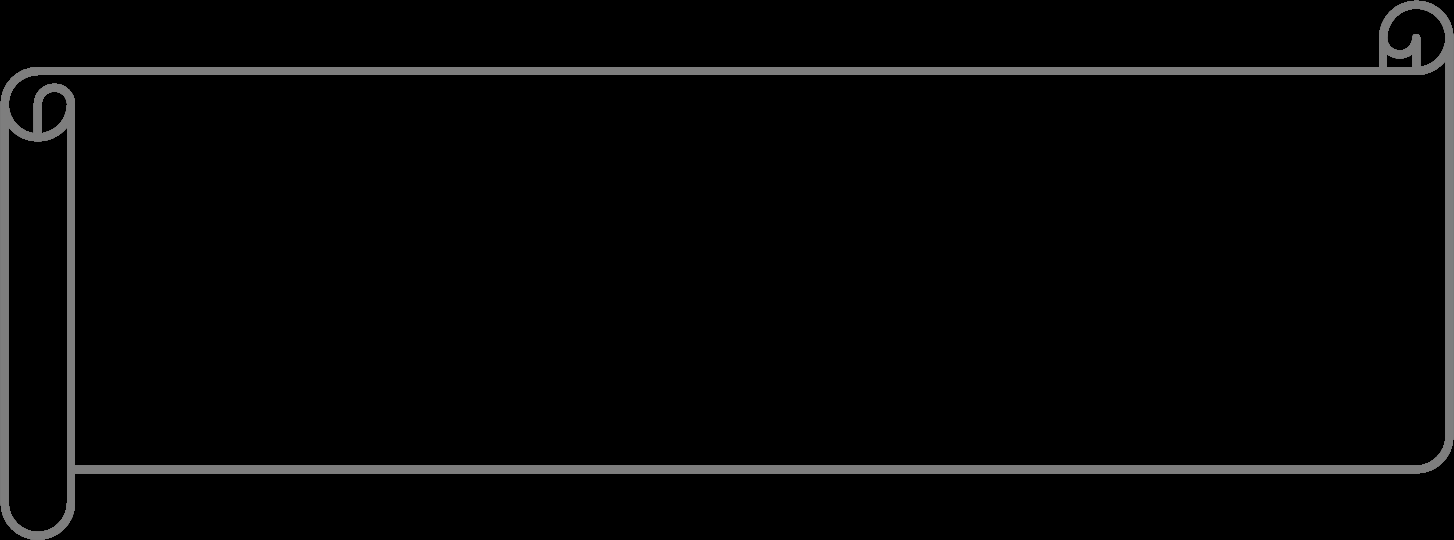
\includegraphics[width=0.4\textwidth]{images/cleaned/logo_emg.png}
        \end{flushleft}
    \end{minipage}
    \begin{minipage}{0.45\textwidth}
        \begin{flushright}
            \textbf{ECOLE MAROCAINE D'INGÉNIERIE}\\
            \small Département Data Science
        \end{flushright}
    \end{minipage}
    
    \vspace{2cm}
    
    {\scshape\Large Rapport de Projet de Fin d'Études (PFE)\par}
    
    \vspace{1.5cm}
    \makebox[\textwidth]{\rule{\textwidth}{1.5pt}}\\[0.5cm]
    {\huge\bfseries Prédiction de la perte de client (Churn) dans le domaine de Télécom\par}
    \vspace{0.2cm}
    {\large\bfseries Application à Telecom Connect\par}
    \makebox[\textwidth]{\rule{\textwidth}{1.5pt}}\\[1.5cm]
    
    \begin{minipage}{0.45\textwidth}
        \begin{flushleft} \large
            \emph{Réalisé par :}\\
            \textbf{Anas Haddou}\\
            \textbf{Mohamed Amine Tayek}
        \end{flushleft}
    \end{minipage}
    \hfill
    \begin{minipage}{0.45\textwidth}
        \begin{flushright} \large
            \emph{Encadré par :}\\
            \textbf{Prof. Noureddine Mohtaram}
        \end{flushright}
    \end{minipage}
    
    \vfill
    {\large Année Universitaire : 2025-2026\par}
\end{titlepage}

% ==========================================
% PAGES PRÉLIMINAIRES
% ==========================================
\pagenumbering{roman}

% Dédicaces
\chapter*{Dédicaces}
\addcontentsline{toc}{chapter}{Dédicaces}
\begin{flushleft}
    \emph{Tout d’abord, nous tenons à remercier ALLAH de nous avoir donné la force et le courage de mener à bien ce modeste travail.}
    
    \vspace{1cm}
    Nous tenons à dédier cet humble travail à :
    \begin{itemize}
        \item Nos tendres mères et nos très chers pères, pour leur amour inconditionnel et leur soutien constant.
        \item Nos précieuses sœurs et nos frères.
        \item Nos chères tantes et nos très chers oncles.
        \item \emph{Spéciale dédicace à vous : Monsieur Rachid Ait Daoud.}
        \item Nos meilleurs amis et tous nos amis d’enfance et du long parcours scolaire et universitaire.
        \item Toutes nos familles et tous ceux qui nous aiment et que nous aimons.
    \end{itemize}
\end{flushleft}

\newpage

% Remerciements
\chapter*{Remerciements}
\addcontentsline{toc}{chapter}{Remerciements}
Nos plus sincères remerciements vont à notre enseignant, \textbf{Mr. Mohtaram}, dont les conseils éclairés et le soutien constant ont été des piliers essentiels tout au long de cette aventure intellectuelle. Ses idées novatrices, ses discussions constructives et ses solutions pertinentes ont profondément enrichi notre travail, témoignant de son engagement envers l'excellence académique.

Un remerciement particulier est adressé à nos familles, dont le soutien indéfectible et la compréhension constante ont été des sources d'inspiration. Leur encouragement a été notre moteur tout au long de nos années d'études.

Enfin, nous n'oublions pas de saluer nos amis d'études et toutes les personnes qui, de près ou de loin, ont contribué à la réalisation de ce projet. Leurs encouragements et leur collaboration ont créé une atmosphère d'apprentissage dynamique et stimulante.

\newpage

% Résumés
\chapter*{Résumé}
\addcontentsline{toc}{chapter}{Résumé}
La perte de clientèle (Churn) représente un défi majeur pour les grandes entreprises, notamment dans le secteur des télécommunications, en raison de son impact direct sur les revenus. Dans ce contexte, la prédiction du churn des clients est cruciale pour anticiper et prévenir cette attrition. Notre travail se concentre sur le développement d'un modèle de prédiction du taux de désabonnement, visant à aider les opérateurs de télécommunications à identifier les clients les plus susceptibles de partir.

Pour atteindre cet objectif, nous avons mis en œuvre plusieurs algorithmes d'apprentissage supervisé et évalué leur performance. Notre principale contribution consiste à développer un modèle performant qui se base sur l'algorithme présentant le meilleur taux de précision. Ce modèle permettra aux opérateurs de télécommunications de prendre des mesures proactives pour réduire le churn et fidéliser leur clientèle.

\vspace{1cm}
\begin{center}
    \rule{0.6\textwidth}{0.5pt}
\end{center}
\vspace{1cm}

\chapter*{Abstract}
\addcontentsline{toc}{chapter}{Abstract}
Customer churn represents a significant challenge for large enterprises, particularly in the telecommunications sector, due to its direct impact on revenue. In this context, predicting customer churn is crucial for anticipating and preventing this attrition. Our work focuses on developing a churn prediction model aimed at helping telecommunications operators identify customers most likely to leave.

To achieve this goal, we implemented various supervised learning algorithms and evaluated their performance. Our main contribution is developing an effective model based on the algorithm with the best accuracy rate. This model will enable telecommunications operators to take proactive measures to reduce churn and retain their customer base.

\newpage

% Tables des matières, figures et tableaux
\tableofcontents
\listoffigures
\listoftables

\newpage

% Abréviations
\chapter*{Abréviations}
\addcontentsline{toc}{chapter}{Abréviations}
\begin{tabular}{ll}
    \textbf{BI} & Business Intelligence \\
    \textbf{CRISP-DM} & Cross-Industry Standard Process for Data Mining \\
    \textbf{JS} & JavaScript \\
    \textbf{HTML} & HyperText Markup Language \\
    \textbf{ML} & Machine Learning \\
    \textbf{DM} & Data Mining \\
    \textbf{IA} & Intelligence Artificielle \\
    \textbf{Churn} & Taux d'attrition des clients \\
    \textbf{CD} & Cahier de Charges \\
    \textbf{DS} & Data Science \\
    \textbf{Sup.} & Supervisé \\
    \textbf{Non-Sup.} & Non Supervisé \\
    \textbf{Admin} & Administrateur \\
\end{tabular}

\newpage

% ==========================================
% CORPS DU RAPPORT
% ==========================================
\pagenumbering{arabic}

\chapter*{Introduction générale}
\addcontentsline{toc}{chapter}{Introduction générale}
Avec l'évolution rapide du secteur des télécommunications, les opérateurs sont confrontés à un défi majeur : la rétention de la clientèle. Dans un contexte où la concurrence est féroce et les consommateurs de plus en plus exigeants, la capacité à anticiper et à prévenir la perte de clients revêt une importance cruciale pour la viabilité économique des entreprises du secteur.

Le présent projet de fin d'études s'inscrit dans ce contexte dynamique en proposant une approche novatrice axée sur la prédiction de la perte de clients dans le domaine des télécommunications. En effet, la capacité à anticiper les comportements des abonnés, en identifiant les signaux précurseurs de résiliation, permet non seulement de minimiser les pertes financières liées à la défection de clients, mais également d'optimiser les efforts de fidélisation.

L'objectif principal de ce rapport est de présenter une méthodologie robuste de prédiction de la perte de client, mettant à profit des techniques avancées d'analyse de données, de machine learning et de modélisation statistique. À travers l'étude approfondie de données historiques, nous nous efforcerons de développer des modèles prédictifs précis et adaptés au contexte spécifique du secteur des télécommunications.

Au-delà de l'aspect technique, ce projet se veut également une réflexion sur les enjeux stratégiques de la fidélisation client dans un marché en perpétuelle mutation. Nous explorerons les implications économiques et opérationnelles de la prédiction de la perte de clients, ainsi que les avantages concurrentiels qu'une telle approche peut conférer aux opérateurs télécoms.

En conclusion, la prédiction de la perte de clients représente une étape stratégique incontournable dans la gestion des relations clientèles pour les entreprises du secteur des télécommunications. Ce projet aspire à contribuer significativement à ce domaine en proposant des solutions innovantes et pragmatiques, ouvrant ainsi la voie à une approche proactive et efficace de la fidélisation dans un environnement télécoms en constante évolution.

% ==========================================
% CHAPITRE 1
% ==========================================
\chapter{CADRE GENERAL DU PROJET}

\section{Introduction}
Dans le secteur des télécommunications, la perte de clients, ou ``churn'', représente un défi majeur en raison de la forte concurrence. Cette problématique entraîne des pertes de revenus et nécessite des investissements considérables pour attirer de nouveaux clients. Afin de prévenir ce phénomène, notre projet se concentre sur le développement d'un modèle de prédiction du churn, utilisant des techniques avancées d'analyse de données et d'apprentissage automatique. En anticipant les départs potentiels, les opérateurs peuvent mettre en place des stratégies proactives pour retenir leur clientèle et maximiser leur rentabilité.

\section{Problématique et Enjeux}
Le churn représente un défi de taille pour les opérateurs télécoms, et ses causes sont variées. Parmi les principales raisons du churn, on retrouve :
\begin{itemize}
    \item \textbf{Insatisfaction du client} : Les clients peuvent être mécontents de divers aspects du service, tels que le prix, la qualité du service client, la couverture réseau, ou encore les fonctionnalités disponibles.
    \item \textbf{Meilleures offres des concurrents} : Lorsque les concurrents proposent des offres plus attrayantes en termes de tarifs, de services ou de fonctionnalités, les clients peuvent être tentés de changer de fournisseur.
    \item \textbf{Manque de communication} : Une communication insuffisante de la part de l'opérateur télécom avec ses clients peut entraîner un sentiment de négligence et de désintérêt, ce qui peut conduire à la perte de confiance et à la volonté de changer de fournisseur.
\end{itemize}

\begin{figure}[H]
    \centering
    
\includegraphics[width=0.6\textwidth]{images/cleaned/figure1_churn.png}
    \caption{Le churn des clients}
    \label{fig:churn_illustr}
\end{figure}

Le churn a des conséquences néfastes sur les résultats financiers des opérateurs télécoms. En effet, outre la perte de revenus directe causée par le départ des clients, le coût associé à l'acquisition de nouveaux clients pour remplacer ceux perdus est souvent élevé. De plus, le churn peut également avoir un impact sur l'image de marque et la réputation de l'opérateur, affectant ainsi sa capacité à attirer de nouveaux clients et à fidéliser les clients existants.

\section{Objectifs spécifiques du projet}
Les entreprises de télécommunications cherchent constamment à réduire leur taux de churn. Pour y parvenir, ce projet vise à développer un modèle de prédiction du churn. Ce modèle analysera les données clients afin d'identifier les facteurs influençant la probabilité de départ. Grâce à ces informations, l'entreprise pourra mettre en place des stratégies de fidélisation ciblées pour les clients à risque, améliorant ainsi la satisfaction client et la rentabilité globale.

\section{Solution proposée}
La solution repose sur l'utilisation de techniques d'apprentissage automatique pour prédire le churn dans le secteur des télécommunications. Nous avons sélectionné des algorithmes tels que la Régression Logistique, les Arbres de Décision, les Random Forests et le Gradient Boosting.

Pour implémenter cette solution, nous utiliserons Python et des bibliothèques comme NumPy, Pandas et Scikit-learn. La visualisation des données sera réalisée avec Matplotlib et Seaborn. Cette approche nous permettra d'identifier les clients à risque de churn, aidant ainsi les entreprises de télécommunications à mettre en place des stratégies de rétention efficaces pour minimiser la perte de clients.

\begin{figure}[H]
    \centering
    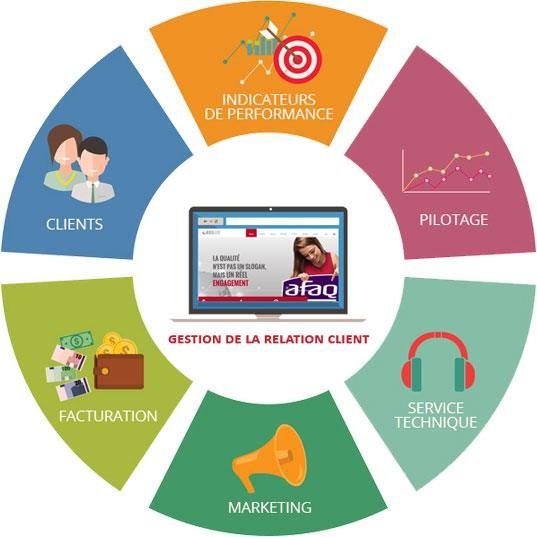
\includegraphics[width=0.5\textwidth]{images/cleaned/figure2_gestion_clienteles.png}
    \caption{La gestion clientèles}
    \label{fig:gestion_clienteles}
\end{figure}

\section{Planification générale du projet}
Le projet sera réalisé en suivant le modèle CRISP-DM et sera divisé en plusieurs phases distinctes :
\begin{enumerate}
    \item \textbf{Compréhension des affaires} : Identifier les objectifs et les exigences du projet.
    \item \textbf{Compréhension des données} : Collecter, décrire et explorer les données disponibles.
    \item \textbf{Préparation des données} : Nettoyer et transformer les données pour les rendre utilisables par les modèles.
    \item \textbf{Modélisation} : Sélectionner et appliquer des techniques de modélisation appropriées.
    \item \textbf{Évaluation} : Évaluer les modèles pour déterminer leur performance et leur pertinence.
    \item \textbf{Déploiement} : Implémenter le modèle dans un environnement opérationnel pour une utilisation réelle.
\end{enumerate}

\begin{figure}[H]
    \centering
    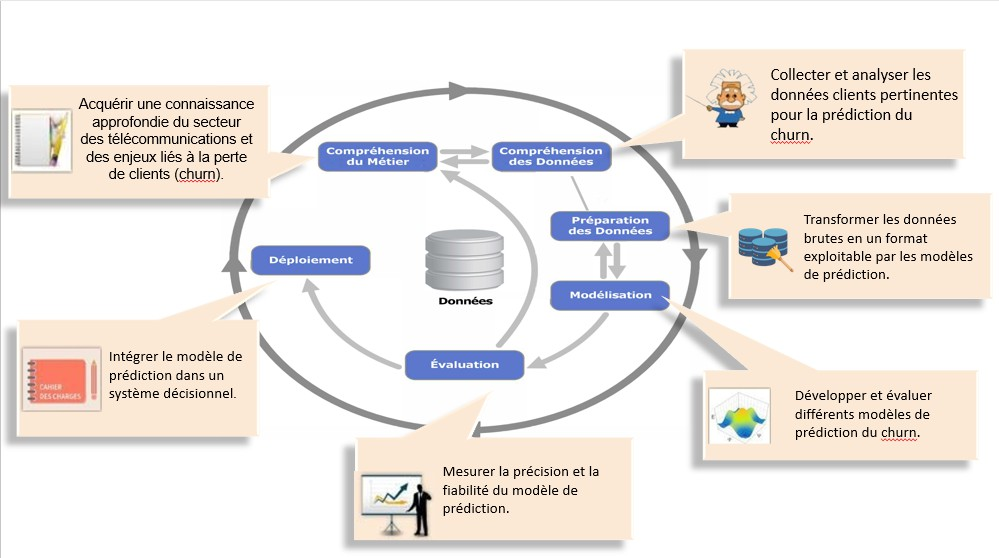
\includegraphics[width=0.7\textwidth]{images/cleaned/figure3_crisp_dm.png}
    \caption{Modèle CRISP-DM}
    \label{fig:crisp_dm}
\end{figure}

\section{Risques et Mesures d'Atténuation}
\subsection{Risques}
\begin{itemize}
    \item \textbf{Disponibilité des données} : Les données clients peuvent ne pas être disponibles ou de qualité insuffisante.
    \item \textbf{Performance du modèle} : Le modèle développé peut manquer de performance et ne pas être en mesure de prédire avec précision le churn.
    \item \textbf{Adoption du modèle} : Le modèle peut ne pas être adopté par les équipes métier, compromettant ainsi son utilité.
\end{itemize}

\subsection{Mesures d'Atténuation}
\begin{itemize}
    \item \textbf{Collecte et Consolidation des Données} : Mettre en place un processus rigoureux de collecte et de consolidation des données clients à partir de différentes sources, afin de garantir leur disponibilité et leur qualité.
    \item \textbf{Choix d'Algorithmes Robustes} : Opter pour des algorithmes d'apprentissage automatique éprouvés et robustes, ayant démontré leur efficacité dans des cas d'utilisation similaires.
    \item \textbf{Implication des Équipes Métier} : Impliquer activement les équipes métier tout au long du développement du modèle, en leur offrant une compréhension approfondie de son fonctionnement.
\end{itemize}

\section{Conclusion}
Le développement d'un modèle de prédiction du churn représente un projet d'une grande importance pour les opérateurs télécoms. Bien que les bénéfices soient significatifs, il est crucial de planifier soigneusement le projet et de prendre en compte les risques potentiels. En adoptant une approche méthodique (CRISP-DM), les opérateurs télécoms peuvent maximiser les chances de succès de leur initiative.

% ==========================================
% CHAPITRE 2
% ==========================================
\chapter{ÉLABORATION DU CAHIER DE CHARGES}

\section{Introduction}
L'objectif des études sur le churn est la détection des individus qui ont l'intention de quitter l'organisation afin d'améliorer la prise de décision et de mettre en place des actions de rétention. La problématique est donc la même pour ces deux phénomènes qui sont souvent analysés à l'aide de techniques prédictives similaires issues du data mining.

\section{Étude de l'existence}
\subsection{Le Data Mining}
Le Data Mining (littéralement ``forage des données'') couvre l'ensemble des outils et méthodes qui permettent d'extraire des connaissances à partir de grandes quantités de données. Il permet à une entreprise de mieux comprendre ses clients, de découvrir des niches rentables, d'optimiser son offre, et de cibler ses actions marketing.

\begin{figure}[H]
    \centering
    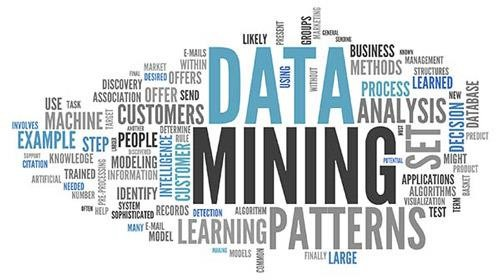
\includegraphics[width=0.6\textwidth]{images/cleaned/figure4_data_mining.png}
    \caption{Le concept de Data Mining}
    \label{fig:data_mining}
\end{figure}

\subsection{Machine Learning}
L'apprentissage automatique (Machine Learning) est une discipline de l'intelligence artificielle qui permet aux ordinateurs d'agir sans être explicitement programmés. Il s'appuie sur des approches mathématiques et statistiques pour permettre aux systèmes d'apprendre à partir des données.

\begin{figure}[H]
    \centering
    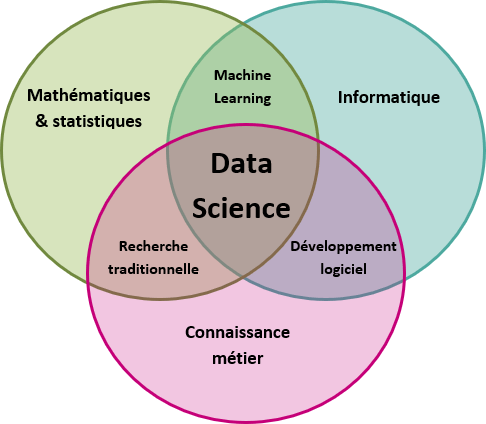
\includegraphics[width=0.5\textwidth]{images/cleaned/figure5_domaine_interdisciplinaire.png}
    \caption{Data Science : une discipline interdisciplinaire}
    \label{fig:data_science_inter}
\end{figure}

On distingue principalement deux types d'apprentissage en Machine Learning :
\begin{itemize}
    \item \textbf{Apprentissage supervisé} : Le modèle est entraîné sur des données étiquetées (ex. classification du churn).
    \item \textbf{Apprentissage non supervisé} : L'ordinateur identifie des modèles sous-jacents sans supervision (ex. segmentation de clients).
\end{itemize}

\begin{figure}[H]
    \centering
    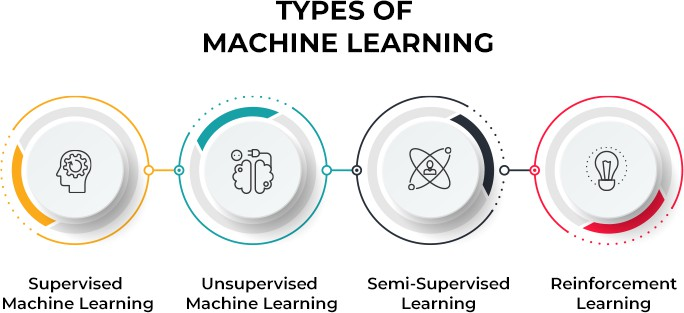
\includegraphics[width=0.6\textwidth]{images/cleaned/figure6_type_machine_learning.png}
    \caption{Types d'apprentissage automatique}
    \label{fig:types_ml}
\end{figure}

\section{Identification des Besoins Fonctionnels et Non Fonctionnels}
\subsection{Besoins Fonctionnels}
\begin{enumerate}
    \item \textbf{Modèle de Prédiction du Churn} : Développer un modèle prédictif basé sur la science des données pour identifier les clients à risque de résiliation.
    \item \textbf{Interface Utilisateur Interactive} : Permettre à un utilisateur de tester un profil de client (prédiction individuelle) ou de charger un fichier CSV pour prédire les résultats en masse (prédiction par lot).
    \item \textbf{Génération de Liste et Exportation} : Exporter les résultats des prédictions en masse dans un format téléchargeable (CSV).
\end{enumerate}

\subsection{Besoins Non Fonctionnels}
\begin{itemize}
    \item \textbf{Précision et Fiabilité} : Le modèle doit être précis pour éviter les faux positifs et faux négatifs coûteux.
    \item \textbf{Performances} : Les temps de traitement pour les prédictions doivent être minimaux.
    \item \textbf{Évolutivité (Scalabilité)} : Possibilité d'intégrer des volumes de données plus importants.
    \item \textbf{Interprétabilité} : Comprendre quels facteurs influencent la décision de résiliation.
    \item \textbf{Facilité d'utilisation} : Une interface ergonomique et intuitive pour les administrateurs et décideurs.
\end{itemize}

\section{Cahier de charges (Exigences des parties)}
Le cahier des charges répond aux besoins de deux rôles principaux :
\begin{itemize}
    \item \textbf{L'administrateur} : Souhaite surveiller et gérer l'application, visualiser les données de churn et configurer les paramètres du système.
    \item \textbf{Le décideur} : Souhaite un accès rapide aux indicateurs clés, la possibilité d'analyser le churn via l'interface et d'extraire des rapports pour orienter la politique commerciale de Telecom Connect.
\end{itemize}

\section{Conclusion}
Ce chapitre a posé les bases conceptuelles et techniques requises pour notre application. En identifiant les besoins fonctionnels et opérationnels, nous avons établi un cadre robuste pour la conception et l'implémentation du système de prédiction.

% ==========================================
% CHAPITRE 3
% ==========================================
\chapter{CONCEPTION DE L'APPLICATION}

\section{Introduction}
Ce chapitre détaille la structure et l'architecture technique de notre application de prédiction du churn. Il aborde le cycle de vie du modèle de Machine Learning, la description des variables du jeu de données, ainsi que le choix des technologies et algorithmes sélectionnés.

\section{Cycle de vie du projet}
Le cycle de vie de notre modèle suit la méthodologie CRISP-DM, allant de la compréhension des objectifs métier à l'évaluation finale et au déploiement.

\begin{figure}[H]
    \centering
    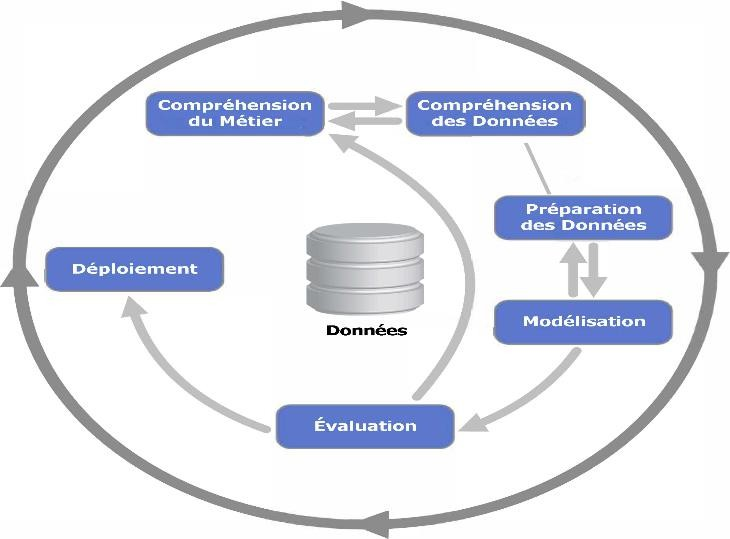
\includegraphics[width=0.6\textwidth]{images/cleaned/figure7_cycle_vie_ml.png}
    \caption{Cycle de vie d'un projet Machine Learning}
    \label{fig:cycle_vie_ml}
\end{figure}

\section{Architecture globale du modèle}
L'architecture de traitement des données comprend plusieurs étapes clés :
\begin{enumerate}
    \item \textbf{Collecte} des données clients.
    \item \textbf{Prétraitement} et nettoyage (encodage, normalisation).
    \item \textbf{Sélection des variables} les plus explicatives.
    \item \textbf{Construction} et entraînement du modèle.
    \item \textbf{Évaluation} et déploiement sous forme d'application Web.
\end{enumerate}

\begin{figure}[H]
    \centering
    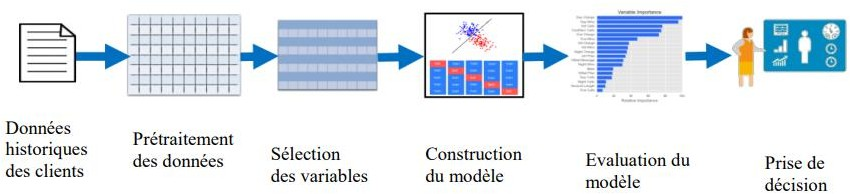
\includegraphics[width=0.7\textwidth]{images/cleaned/figure8_architecture_modele.png}
    \caption{Architecture globale du modèle}
    \label{fig:arch_modele}
\end{figure}

\section{Jeu de Données (Dataset)}
Pour cette étude, nous utilisons un dataset de télécommunications disponible sur Kaggle, qui contient \textbf{7043 lignes} (clients) et \textbf{21 variables}.

Le Tableau \ref{tab:variables} présente la description détaillée des variables explicatives clés :

\begin{table}[H]
\centering
\caption{Description des variables clés du Dataset}
\label{tab:variables}
\small
\begin{tabular}{llcc}
\toprule
\textbf{Variable} & \textbf{Description} & \textbf{Valeurs Uniques} & \textbf{Type} \\
\midrule
GENDER & Sexe du client & 2 & Object \\
SENIORCITIZEN & Si le client est une personne âgée (0/1) & 2 & Int64 \\
PARTNER & Si le client a un partenaire (Oui/Non) & 2 & Object \\
DEPENDENTS & Nombre de personnes à charge du client & 2 & Object \\
TENURE & Nombre de mois d'ancienneté du client & 73 & Int64 \\
PHONESERVICE & Service téléphonique activé (Oui/Non) & 2 & Object \\
MULTIPLELINES & Plusieurs lignes téléphoniques (Oui/Non/Sans) & 3 & Object \\
INTERNETSERVICE & Type de service Internet (DSL, Fibre, Non) & 3 & Object \\
ONLINESECURITY & Service de sécurité en ligne activé & 3 & Object \\
ONLINEBACKUP & Service de sauvegarde en ligne activé & 3 & Object \\
DEVICEPROTECTION & Service de protection des appareils activé & 3 & Object \\
TECHSUPPORT & Service d'assistance technique activé & 3 & Object \\
STREAMINGTV & Service de streaming TV activé & 3 & Object \\
STREAMINGMOVIES & Service de streaming de films activé & 3 & Object \\
CONTRACT & Durée du contrat (Mois, Un an, Deux ans) & 3 & Object \\
PAPERLESSBILLING & Facturation sans papier (Oui/Non) & 2 & Object \\
PAYMENTMETHOD & Mode de paiement (Chèque, Carte, Virement) & 4 & Object \\
MONTHLYCHARGES & Frais mensuels pour les services & 1585 & Float64 \\
TOTALCHARGES & Total des frais payés par le client & 6531 & Float64 \\
CHURN (Cible) & Si le client a résilié le mois dernier & 2 & Object \\
\bottomrule
\end{tabular}
\end{table}

\section{Choix des algorithmes et technologies}
\subsection{Algorithmes de Classification}
Cinq algorithmes principaux ont été mis en compétition :
\begin{itemize}
    \item \textbf{Random Forest Classifier} : Algorithme d'ensemble qui crée de multiples arbres de décision pour une classification robuste.
    \item \textbf{Gradient Boosting Classifier} : Modélisation séquentielle corrigeant les erreurs des arbres précédents.
    \item \textbf{Régression Logistique} : Modèle de référence pour la classification binaire.
    \item \textbf{Support Vector Classifier (SVC)} : Maximise la marge de séparation entre les classes.
    \item \textbf{Decision Tree Classifier} : Modèle d'arbre simple et facilement interprétable.
\end{itemize}

\subsection{Technologies logicielles}
\begin{itemize}
    \item \textbf{Python} : Langage principal pour la science des données.
    \item \textbf{Flask} : Framework léger pour la création de l'application Web.
    \item \textbf{Pandas \& NumPy} : Manipulation et calcul numérique.
    \item \textbf{Scikit-learn} : Pipeline de machine learning et évaluation des modèles.
    \item \textbf{Matplotlib \& Seaborn} : Visualisations graphiques.
    \item \textbf{PythonAnywhere} : Plateforme choisie pour héberger l'application Web.
\end{itemize}

\section{Interface Utilisateur}
L'application Web comprend deux fonctionnalités principales pour la prédiction :
\begin{enumerate}
    \item \textbf{Prédiction individuelle} : Formulaire Web interactif pour entrer les données d'un client unique.
    \item \textbf{Prédiction par lot (Batch)} : Zone de dépôt de fichier CSV pour analyser plusieurs profils clients en une seule fois.
\end{enumerate}

\begin{figure}[H]
    \centering
    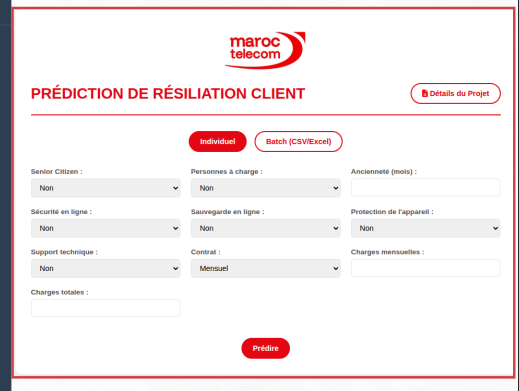
\includegraphics[width=0.6\textwidth]{images/cleaned/figure9_prediction_individuelle.png}
    \caption{Interface de Prédiction pour un seul client}
    \label{fig:ui_single}
\end{figure}

\begin{figure}[H]
    \centering
    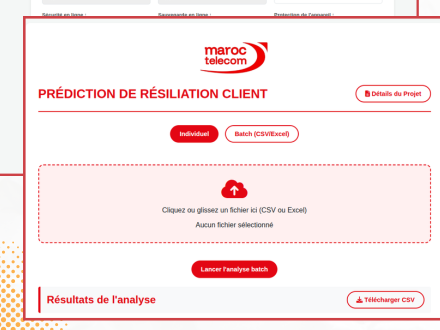
\includegraphics[width=0.6\textwidth]{images/cleaned/figure10_prediction_groupe.png}
    \caption{Interface de Prédiction pour un groupe de clients}
    \label{fig:ui_batch}
\end{figure}

\section{Conclusion}
La conception technique définit clairement le flux d'informations et l'ergonomie de l'outil Web. Ce travail préparatoire assure une transition sans encombre vers la phase de développement et d'implémentation.

% ==========================================
% CHAPITRE 4
% ==========================================
\chapter{DÉVELOPPEMENT ET IMPLÉMENTATION}

\section{Introduction}
Ce chapitre présente la mise en œuvre pratique de la solution de prédiction, depuis le nettoyage des données brutes jusqu'au déploiement Web sur PythonAnywhere.

\section{Compréhension et Nettoyage des données}
Lors de la phase d'analyse exploratoire des données (EDA), la structure du dataset a été vérifiée à l'aide de la commande \texttt{df.info()}.

\begin{figure}[H]
    \centering
    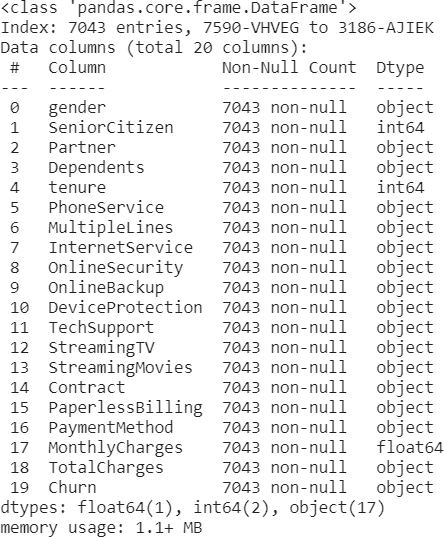
\includegraphics[width=0.45\textwidth]{images/cleaned/figure11_resume_donnees.png}
    \caption{Structure du Dataset de Churn}
    \label{fig:dataset_info}
\end{figure}

Bien que le dataset ne présente aucune valeur explicitement nulle à l'origine, nous avons constaté que la variable \texttt{TotalCharges} était incorrectement typée en tant qu'objet (\texttt{object}) au lieu d'une variable numérique. Cela s'explique par la présence d'espaces vides pour certains nouveaux clients.

Pour y remédier, le script de traitement convertit ces valeurs en types numériques et remplace les espaces par des valeurs \texttt{NaN} :
\begin{lstlisting}[language=Python, caption=Conversion de TotalCharges en type numérique]
# Modification du type de la colonne TotalCharges
df["TotalCharges"] = pd.to_numeric(df["TotalCharges"], errors="coerce")
\end{lstlisting}

Après cette conversion, 11 valeurs manquantes ont été identifiées dans la colonne \texttt{TotalCharges}. Compte tenu de leur faible volume, nous avons procédé à la suppression des lignes correspondantes.

\section{Modélisation et Entraînement}
Les données ont été séparées en un jeu d'entraînement (80\%) et un jeu de test (20\%). Nous avons entraîné chaque modèle de classification et ajusté manuellement les hyperparamètres afin d'obtenir la meilleure capacité de généralisation.

Le code d'implémentation de l'algorithme de Forêt d'Arbres Décisionnels (Random Forest) est illustré ci-dessous :
\begin{lstlisting}[language=Python, caption=Entrainement du modèle Random Forest]
from sklearn.ensemble import RandomForestClassifier
from sklearn.metrics import accuracy_score, confusion_matrix, classification_report

# Initialisation avec des hyperparametres optimisés
Rfc = RandomForestClassifier(n_estimators=120, criterion='gini', max_depth=15, 
                             min_samples_leaf=10, min_samples_split=5)
Rfc.fit(x_train, y_train)
rfc_pred = Rfc.predict(x_test)

print(f'Accuracy score : {accuracy_score(rfc_pred, y_test)}')
print(f'Confusion matrix :\n {confusion_matrix(rfc_pred, y_test)}')
\end{lstlisting}

\section{Évaluation des Modèles}
Les modèles entraînés ont été évalués à l'aide de diverses métriques : l'exactitude (Accuracy), le rappel (Recall), la précision (Precision), le score F1 (f1-score), l'aire sous la courbe ROC (Roc\_auc) et le coefficient Kappa de Cohen (Kappa\_metric).

Le Tableau \ref{tab:metrics} résume la comparaison de performance des différents modèles testés :

\begin{table}[H]
\centering
\caption{Comparaison des performances des modèles de Machine Learning}
\label{tab:metrics}
\small
\begin{tabular}{lcccccc}
\toprule
\textbf{Modèle} & \textbf{Accuracy} & \textbf{Recall} & \textbf{Precision} & \textbf{F1-score} & \textbf{ROC AUC} & \textbf{Kappa} \\
\midrule
Logistic (Baseline) & 0.9099 & 0.9386 & 0.8909 & 0.9141 & 0.9093 & 0.8195 \\
Decision Tree & 0.9437 & 0.9480 & 0.9421 & 0.9451 & 0.9436 & 0.8873 \\
\textbf{Random Forest} & \textbf{0.9590} & \textbf{0.9717} & \textbf{0.9492} & \textbf{0.9603} & \textbf{0.9587} & \textbf{0.9179} \\
SVM (linear) & 0.9155 & 0.9402 & 0.8991 & 0.9192 & 0.9150 & 0.8308 \\
Gradient Boosting & 0.9590 & 0.9654 & 0.9548 & 0.9601 & 0.9588 & 0.9179 \\
\bottomrule
\end{tabular}
\end{table}

\begin{figure}[H]
    \centering
    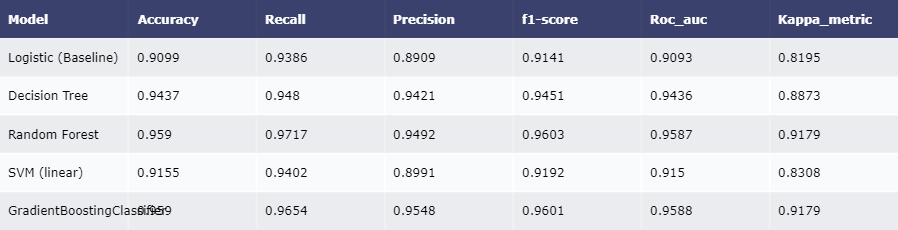
\includegraphics[width=0.85\textwidth]{images/cleaned/figure14_confusion_matrices.png}
    \caption{Matrices de confusion des modèles évalués}
    \label{fig:confusion_matrices}
\end{figure}

Le modèle \textbf{Random Forest} affiche des performances optimales avec une exactitude de \textbf{95.90\%} et un excellent coefficient Kappa de \textbf{0.9179}, ce qui indique une prédiction très fiable, confirmée par la matrice de confusion.

\section{Déploiement du Modèle}
Pour le déploiement Web, nous avons choisi la plateforme \textbf{PythonAnywhere} en suivant les étapes clés :
\begin{enumerate}
    \item Choix de la plateforme d'hébergement.
    \item Configuration de l'application Flask et chargement des fichiers de sérialisation (\texttt{pickle}) contenant le modèle et les transformations de données.
    \item Configuration de l'environnement virtuel pour installer les dépendances nécessaires.
    \item Publication de l'application Web accessible via une URL publique dédiée.
\end{enumerate}

\section{Conclusion}
La phase de développement a permis de concrétiser le pipeline de données. Les excellents résultats obtenus par le modèle Random Forest confortent sa sélection pour alimenter l'interface de prédiction de Telecom Connect.

% ==========================================
% CHAPITRE 5
% ==========================================
\chapter{RESULTATS ET DISCUSSION}

\section{Introduction}
Ce chapitre analyse l'intégration du modèle au sein de l'application Web interactive et discute de l'influence des différentes variables sur le phénomène de désabonnement, tout en mettant en lumière les limites et pistes d'amélioration du projet.

\section{Résultats de l'application Web}
L'application Flask propose un affichage convivial des prédictions. L'utilisateur peut renseigner les données du formulaire individuel pour obtenir instantanément le statut estimé du client.

\begin{figure}[H]
    \centering
    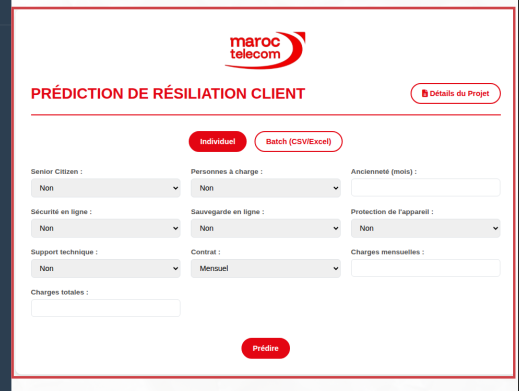
\includegraphics[width=0.6\textwidth]{images/cleaned/figure15_interface_prediction_client.png}
    \caption{Visualisation du résultat d'une prédiction individuelle}
    \label{fig:res_single}
\end{figure}

Pour l'analyse en masse, l'administrateur dépose un fichier CSV et l'application renvoie un tableau contenant la prédiction associée à chaque profil client (soit ``Churn'' en rouge, soit ``Fidèle'' en vert), avec une option d'exportation vers un nouveau fichier CSV.

\begin{figure}[H]
    \centering
    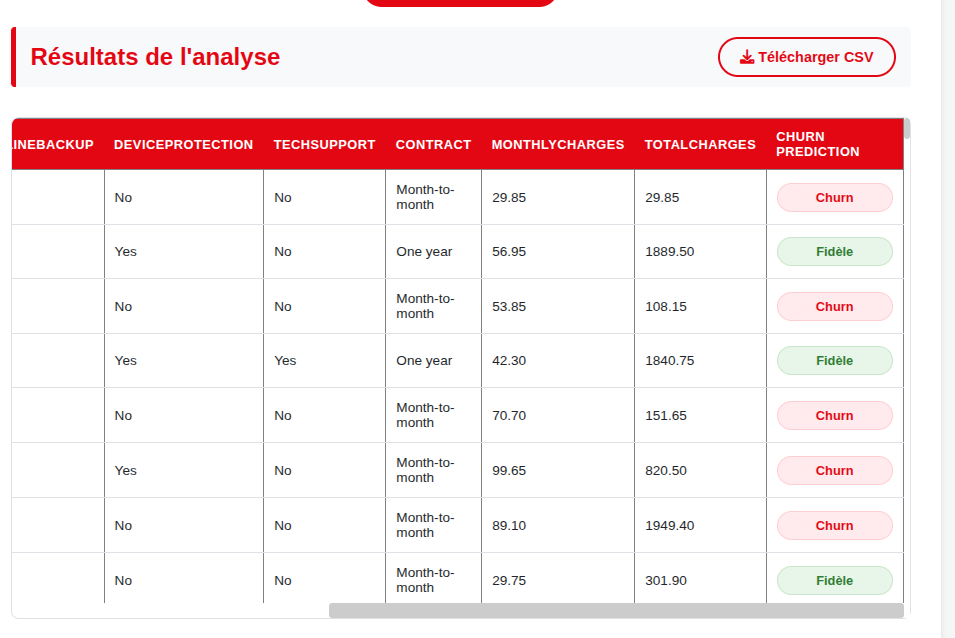
\includegraphics[width=0.8\textwidth]{images/cleaned/figure16_prediction_plusieurs_clients.png}
    \caption{Visualisation des prédictions par lot (Batch)}
    \label{fig:res_batch}
\end{figure}

\section{Facteurs déterminants du Churn}
Une analyse de corrélation a été menée pour identifier les facteurs jouant un rôle prépondérant dans la résiliation des clients.

\begin{figure}[H]
    \centering
    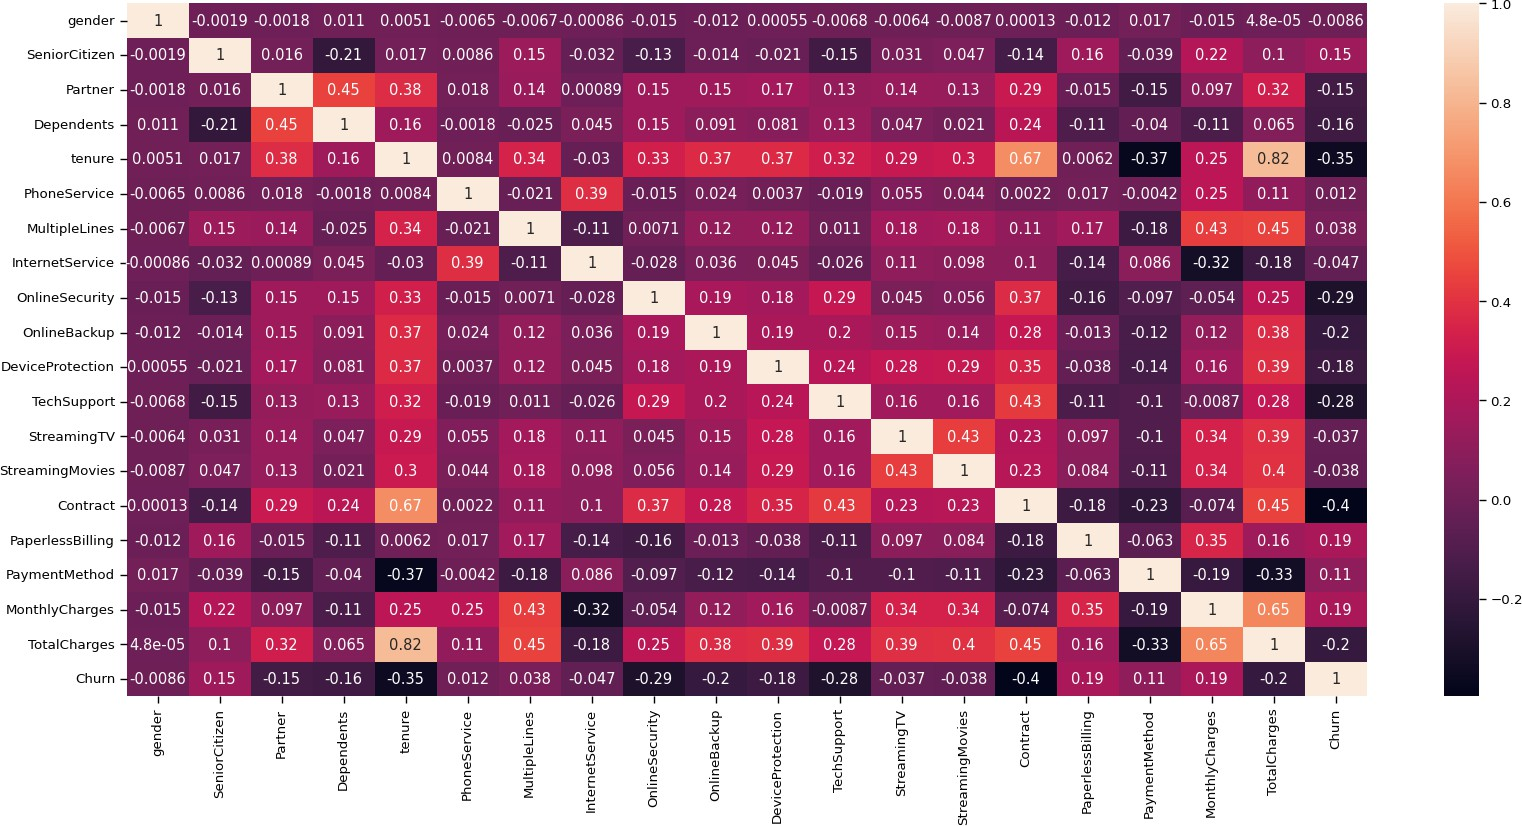
\includegraphics[width=0.85\textwidth]{images/cleaned/figure17_facteurs_determinants.png}
    \caption{Matrice de corrélation des fonctionnalités}
    \label{fig:correlation}
\end{figure}

Les facteurs les plus critiques identifiés sont :
\begin{itemize}
    \item \textbf{Le type de contrat} : Les contrats au mois le mois affichent une corrélation positive très forte avec le churn, par opposition aux engagements sur un ou deux ans.
    \item \textbf{La durée d'ancienneté (Tenure)} : Plus le client est ancien, moins il est enclin à résilier son contrat.
    \item \textbf{Les frais mensuels (Monthly Charges)} : Des tarifs élevés contribuent à une augmentation de la probabilité de désabonnement.
    \item \textbf{Les services d'assistance} : L'absence de support technique (\texttt{TechSupport}) ou de sécurité en ligne (\texttt{OnlineSecurity}) favorise le churn.
\end{itemize}

\section{Limitations du modèle}
Bien que le modèle Random Forest soit particulièrement performant, nous notons certaines limites :
\begin{itemize}
    \item \textbf{Qualité et quantité des données} : Le dataset de 7043 clients provient d'un échantillon fixe. Un historique plus récent et volumineux permettrait de capturer les nouvelles tendances du marché.
    \item \textbf{Risque de surapprentissage} : Le réglage précis sur le dataset actuel nécessite des mises à jour régulières pour éviter que le modèle ne perde en généralisation sur de nouveaux profils clients.
    \item \textbf{Variables non prises en compte} : Des données externes telles que les pannes réseau, les plaintes au service client ou les offres des concurrents directs n'ont pas pu être intégrées dans le modèle.
\end{itemize}

\section{Pistes d'Amélioration}
\begin{itemize}
    \item \textbf{Collecte continue} : Intégrer un flux de données en temps réel pour ré-entraîner périodiquement le modèle.
    \item \textbf{Ajout de fonctionnalités d'interaction} : Prendre en compte le nombre d'appels passés au support technique ou l'historique des réclamations.
    \item \textbf{Optimisation automatique des hyperparamètres} : Utiliser des techniques comme \texttt{GridSearchCV} ou \texttt{RandomizedSearchCV}.
\end{itemize}

\section{Conclusion}
Le système développé fournit des résultats robustes et immédiatement exploitables par Telecom Connect. L'identification des facteurs clés, tels que le type de contrat et la présence de services d'assistance, offre des leviers d'action concrets pour fidéliser la clientèle.

% ==========================================
% CONCLUSION GENERALE
% ==========================================
\chapter*{Conclusion et perspectives}
\addcontentsline{toc}{chapter}{Conclusion et perspectives}
En conclusion, ce projet de fin d'études a permis de concevoir et de déployer une solution complète de prédiction de la perte de clientèle (Churn) pour Telecom Connect. En suivant la méthodologie CRISP-DM, nous avons mené à bien l'analyse exploratoire, le nettoyage des données, ainsi que l'entraînement et l'évaluation de plusieurs modèles de classification.

Nos résultats démontrent que l'utilisation du modèle \textbf{Random Forest Classifier} permet d'atteindre un taux d'exactitude de \textbf{95.90\%}, offrant ainsi aux décideurs un outil d'aide à la décision fiable et performant. Grâce à l'interface Web développée sous Flask et déployée sur PythonAnywhere, l'application est facilement accessible et utilisable pour tester des profils clients de manière individuelle ou par lot.

\subsection*{Perspectives d'avenir}
\begin{enumerate}
    \item \textbf{Intégration d'un tableau de bord décisionnel} : Développer un module BI interactif avec des visualisations dynamiques en temps réel du taux de churn global et de la répartition géographique.
    \item \textbf{Analyse des sentiments} : Connecter le modèle à un outil d'analyse des avis clients sur les réseaux sociaux et des transcriptions d'appels pour anticiper le mécontentement.
    \item \textbf{Système de recommandation d'offres} : Proposer automatiquement au conseiller clientèle une offre promotionnelle ou un service de rétention adapté au profil du client à risque identifié.
\end{enumerate}

Le churn est un défi permanent, mais l'adoption d'approches prédictives basées sur le Machine Learning permet aux entreprises de télécommunications de passer d'une posture réactive à une stratégie proactive de fidélisation de leur clientèle.

% ==========================================
% BIBLIOGRAPHIE
% ==========================================
\chapter*{Bibliographie \& Webographie}
\addcontentsline{toc}{chapter}{Bibliographie \& Webographie}
\begin{enumerate}
    \item Google Scholar - \emph{Prédiction du churn des clients dans les télécommunications}.
    \item Kaggle - \emph{Telecom Customer Churn Dataset} (\url{https://www.kaggle.com}).
    \item Scikit-Learn Documentation - \emph{Random Forest Classifier \& Machine Learning Evaluation Metrics}.
    \item Flask Framework Documentation - \emph{Web Deployment with Python}.
    \item Ooredoo Research Center - \emph{Churn prediction methodologies}.
    \item ASJP (Algerian Scientific Journal Platform) - \emph{L'importance du Data Mining dans le secteur des services}.
    \item BASE (Bielefeld Academic Search Engine) - \emph{Academic papers on churn classification}.
    \item OATD (Open Access Theses and Dissertations) - \emph{Customer retention and machine learning applications}.
    \item PythonAnywhere Web Hosting Guide - \emph{WSGI configuration for Flask applications}.
\end{enumerate}

\end{document}
